\chapter{Conceptual and Technical Architecture}
\begin{spacing}{1.2}
\minitoc
\thispagestyle{MyStyle}
\end{spacing}
\newpage

\section*{INTRODUCTION}
\addcontentsline{toc}{section}{INTRODUCTION}
This chapter presents the conceptual and technical architecture of Itqan: the four-layer architecture and four-pillar map (§4.1), the BACAB layered pattern (§4.2), the manager service's three-gate lifecycle (§4.3), the trust-boundary architecture of the copilot (§4.4), the evidence boundary (§4.5), and the platform-integration view and ADR register (§4.6).

\section{Global Architecture and Four-Pillar Layering}
Itqan is organised at the platform level into four layers and conceived as four capability pillars. Layers describe \textit{how} components are arranged, pillars describe \textit{what} capabilities they realise; the RFQ Copilot sits across both views as a cross-cutting interaction consumer rather than as a fifth layer or pillar.

\subsection{The Four Architectural Layers and the Cross-Cutting Copilot}
The \textbf{presentation layer} is the user interface service; the \textbf{orchestration layer} is the manager service, which owns lifecycle representation and operational truth; the \textbf{intelligence layer} is the intelligence service, which produces deterministic analytical artifacts without owning lifecycle state; the \textbf{data layer} comprises the persistence stores managed by each service, kept private to its owner so that the boundaries remain enforceable. The \textbf{RFQ Copilot} owns no lifecycle, document, or analytical truth; it queries, explains, and safely exposes the evidence produced by the manager and intelligence services, traversing the presentation, orchestration, and intelligence layers as a cross-cutting consumer. Its internal trust-boundary architecture is developed in Section~4.4. Figure~\ref{fig:itqan_global} presents the layered architecture with the copilot's cross-cutting position.

\begin{figure}[H]
    \centering
    \setlength{\fboxsep}{5pt}
    \setlength{\fboxrule}{0.5pt}
    \fbox{
        \IfFileExists{images/fig_4_1_itqan_global.png}{%
            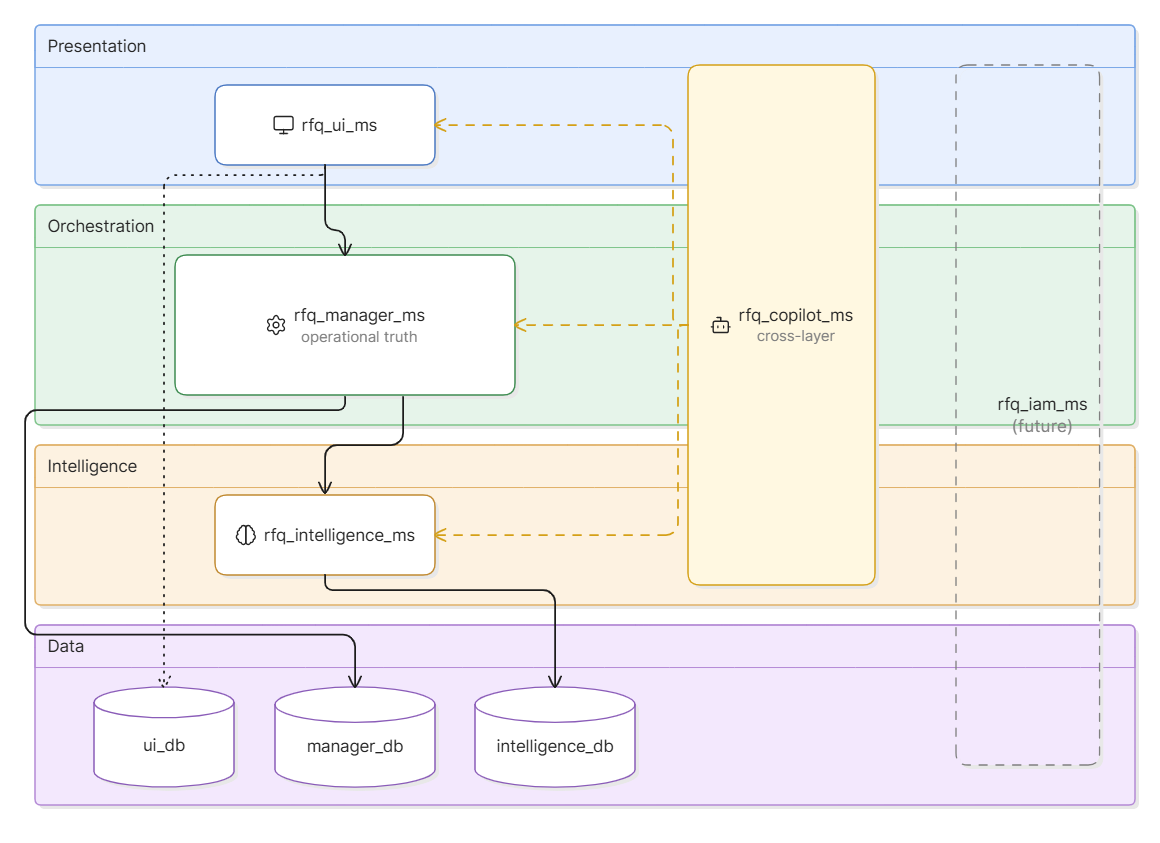
\includegraphics[width=\linewidth]{images/fig_4_1_itqan_global.png}%
        }{%
            \begin{minipage}[c][8cm][c]{14cm}
                \centering
                \textit{[Figure 4.1 placeholder: Itqan global architecture showing the four layers (presentation, orchestration, intelligence, data), the four implemented services and the future-scope IAM service, and the cross-cutting position of the RFQ Copilot as a consumer that traverses presentation, orchestration, and intelligence without owning data.]}
            \end{minipage}%
        }
    }
    \caption{Global architecture of the Itqan platform: four layers, services, and the cross-cutting position of the RFQ Copilot}
    \label{fig:itqan_global}
\end{figure}

\subsection{The Four Pillars as an Architectural Map}
The four pillars introduced in Chapter~1 each map to a primary owning service: \textbf{Workflow and Tracking} to the manager service; \textbf{Communication Automation} also to the manager service through reminder infrastructure (outbound channels and inbound monitoring remain future scope); \textbf{Executive Intelligence and BI} co-owned by the manager service (aggregations) and the user interface (dashboards); \textbf{Historical Learning and Prediction} to the intelligence service at the deterministic-parsing level, with predictive components deferred. Table~\ref{tab:pillar_scope} presents the scope status of each pillar.

\begin{table}[H]
\centering
\renewcommand{\arraystretch}{1.4}
\begin{tabularx}{\textwidth}{|p{3.5cm}|p{2.3cm}|>{\RaggedRight\arraybackslash}X|}
\hline
\rowcolor{lightgray}
\textbf{Pillar} & \textbf{Status} & \textbf{Notes on Coverage} \\ \hline
Workflow and Tracking & Implemented & Operational backbone of the platform, delivered through the manager service across all primary lifecycle resources. \\ \hline
Communication Automation & Partial & Reminder infrastructure delivered inside the manager service; outbound delivery channels, inbound monitoring, and assisted drafting remain future capabilities, not a separate microservice in the present scope. \\ \hline
Executive Intelligence and BI & Partial & Analytical endpoints delivered in the manager service; demonstration dashboards consumed by the UI; full BI surface, including profitability and competitive analysis, is future scope. \\ \hline
Historical Learning and Prediction & Foundation only & Deterministic parsing of MR packages and estimation workbooks delivered in the intelligence service; pattern matching, supplier intelligence, and predictive components are future scope. \\ \hline
\end{tabularx}
\caption{Scope status of the four pillars at the conclusion of the present work}
\label{tab:pillar_scope}
\end{table}

\section{Microservices Inventory and BACAB Pattern}
\subsection{Service Inventory}
The platform is organised around \textbf{five services} --- four implemented or partial, one deferred. \texttt{rfq\_manager\_ms} is the lifecycle backbone and most mature implementation. \texttt{rfq\_copilot\_ms} is the trust-bound conversational layer, with its first vertical slice shipped. \texttt{rfq\_intelligence\_ms} is implemented at the foundation level for the Chapter~2 parsing scope. \texttt{rfq\_ui\_ms} is an interface layer with live API support and demo/mock fallback; browser end-to-end validation is pending. \texttt{rfq\_iam\_ms} is future scope; the manager service carries a built IAM integration point (bearer-token path and identity-resolution connector) for that service to slot into. Service boundaries follow data ownership: the manager owns lifecycle state, the intelligence service owns analytical artifacts, the copilot owns conversation state only, and the user interface owns presentation logic. This ownership discipline is what makes the trust-boundary architecture of Section~4.4 possible: because the copilot owns no operational truth, its answers must remain mediated by the services that do.

\subsection{The BACAB Layered Pattern}
Inside each backend service, the code follows the \hostCompany{} layered convention adapted to this platform. Five \textbf{active layers} carry the request path --- \texttt{routes} (HTTP entry and input validation), \texttt{controllers} (business logic), \texttt{datasources} (persistence boundary), \texttt{translators} (cross-boundary shape conversion), and \texttt{connectors} (external-service calls including the language-model API for the copilot) --- supported transversally by three layers: \texttt{models}, \texttt{config}, and \texttt{utils}. Three discipline rules hold throughout: routes do not contain business logic; controllers do not access the database directly; datasources do not make decisions. Figure~\ref{fig:bacab_pattern} presents the structure. The copilot service preserves this skeleton at the HTTP/data layer and adds a dedicated \texttt{pipeline} layer for the per-turn stages of Section~4.4.

\begin{figure}[H]
    \centering
    \setlength{\fboxsep}{5pt}
    \setlength{\fboxrule}{0.5pt}
    \fbox{
        \IfFileExists{images/fig_4_2_bacab_pattern.png}{%
            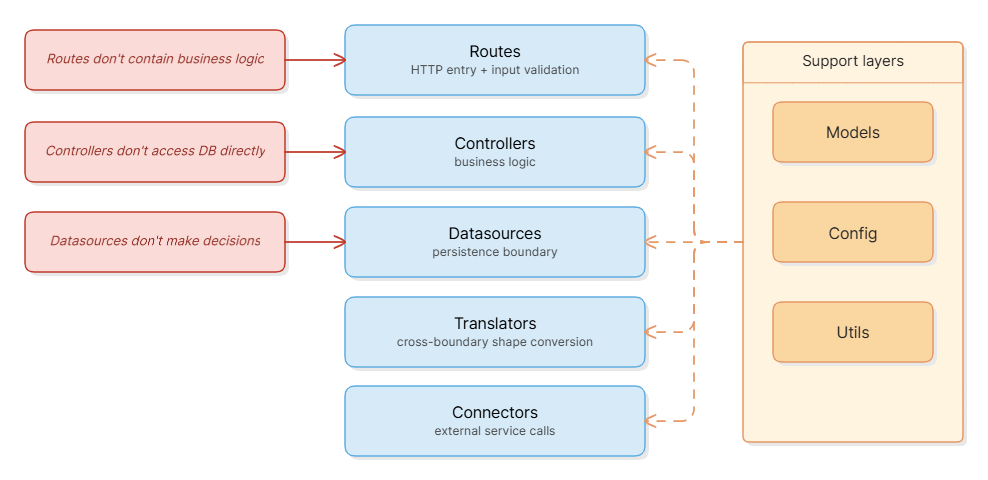
\includegraphics[width=\linewidth]{images/fig_4_2_bacab_pattern.png}%
        }{%
            \begin{minipage}[c][7cm][c]{14cm}
                \centering
                \textit{[Figure 4.2 placeholder: BACAB layered pattern. Five active layers shown vertically in request-path order (Routes $\rightarrow$ Controllers $\rightarrow$ Datasources $\rightarrow$ Translators $\rightarrow$ Connectors), three support layers (Models, Config, Utils) shown as a sidebar serving the active layers, with the three discipline rules annotated.]}
            \end{minipage}%
        }
    }
    \caption{The BACAB layered pattern: five active layers in request-path order, three support layers, three discipline rules}
    \label{fig:bacab_pattern}
\end{figure}

\subsection{Inter-Service Communication}
Inter-service communication follows three conventions. \textit{Contracts:} synchronous REST over HTTP, each service publishing an OpenAPI specification with explicit path-level versioning as the single source of truth. \textit{Errors:} a consistent structured shape (HTTP status code, machine-readable error type, human-readable message) with authorisation outcomes distinguished (\texttt{401} unauthenticated, \texttt{403} authenticated but unauthorised, \texttt{404} for resources the user is not permitted to know exist); the manager service emits a per-request correlation identifier, with uniform cross-service propagation as a hardening direction. \textit{Access:} the copilot never bypasses manager-mediated access --- every retrieval of lifecycle data goes through the manager's authorised endpoints with actor context propagated explicitly, the convention Section~4.4 revisits as the access boundary of the trust-bound architecture.

\section{Manager Service: Domain Model and Lifecycle}

\subsection{Mission and Domain Model}
The manager service is the operational backbone of the platform: it maintains a structured, observable representation of every RFQ and enforces the rules that govern lifecycle progression. Its mission is deliberately constrained --- estimation remains with senior estimators per Chapter~1, and analytical intelligence is produced by the intelligence service. The domain model is organised around seven primary entities (Figure~\ref{fig:manager_erd}): the \textbf{RFQ} (root, with identifying metadata, classification, source channel, current lifecycle status); the \textbf{Workflow} (versioned stage-sequence template, instantiated per RFQ); the \textbf{RFQ\_Stage} (per-RFQ stage instance carrying progression state, mandatory fields, computed transition rules); the \textbf{Subtask} (finer-grained unit attached to a stage, with soft-delete semantics and parent progress propagation); the \textbf{Note} (append-only textual artifact); the \textbf{File} (persisted document, including the estimation workbook once uploaded); and the \textbf{Reminder} (time-anchored notification, manual or rule-based). Five auxiliary tables (templates, rule definitions, code counters, per-field stage values, reserved audit-history shape) complete the schema and are detailed in Chapter~5 (Section~5.2.2).

\begin{figure}[H]
    \centering
    \setlength{\fboxsep}{5pt}
    \setlength{\fboxrule}{0.5pt}
    \fbox{
        \IfFileExists{images/fig_4_3_manager_erd.png}{%
            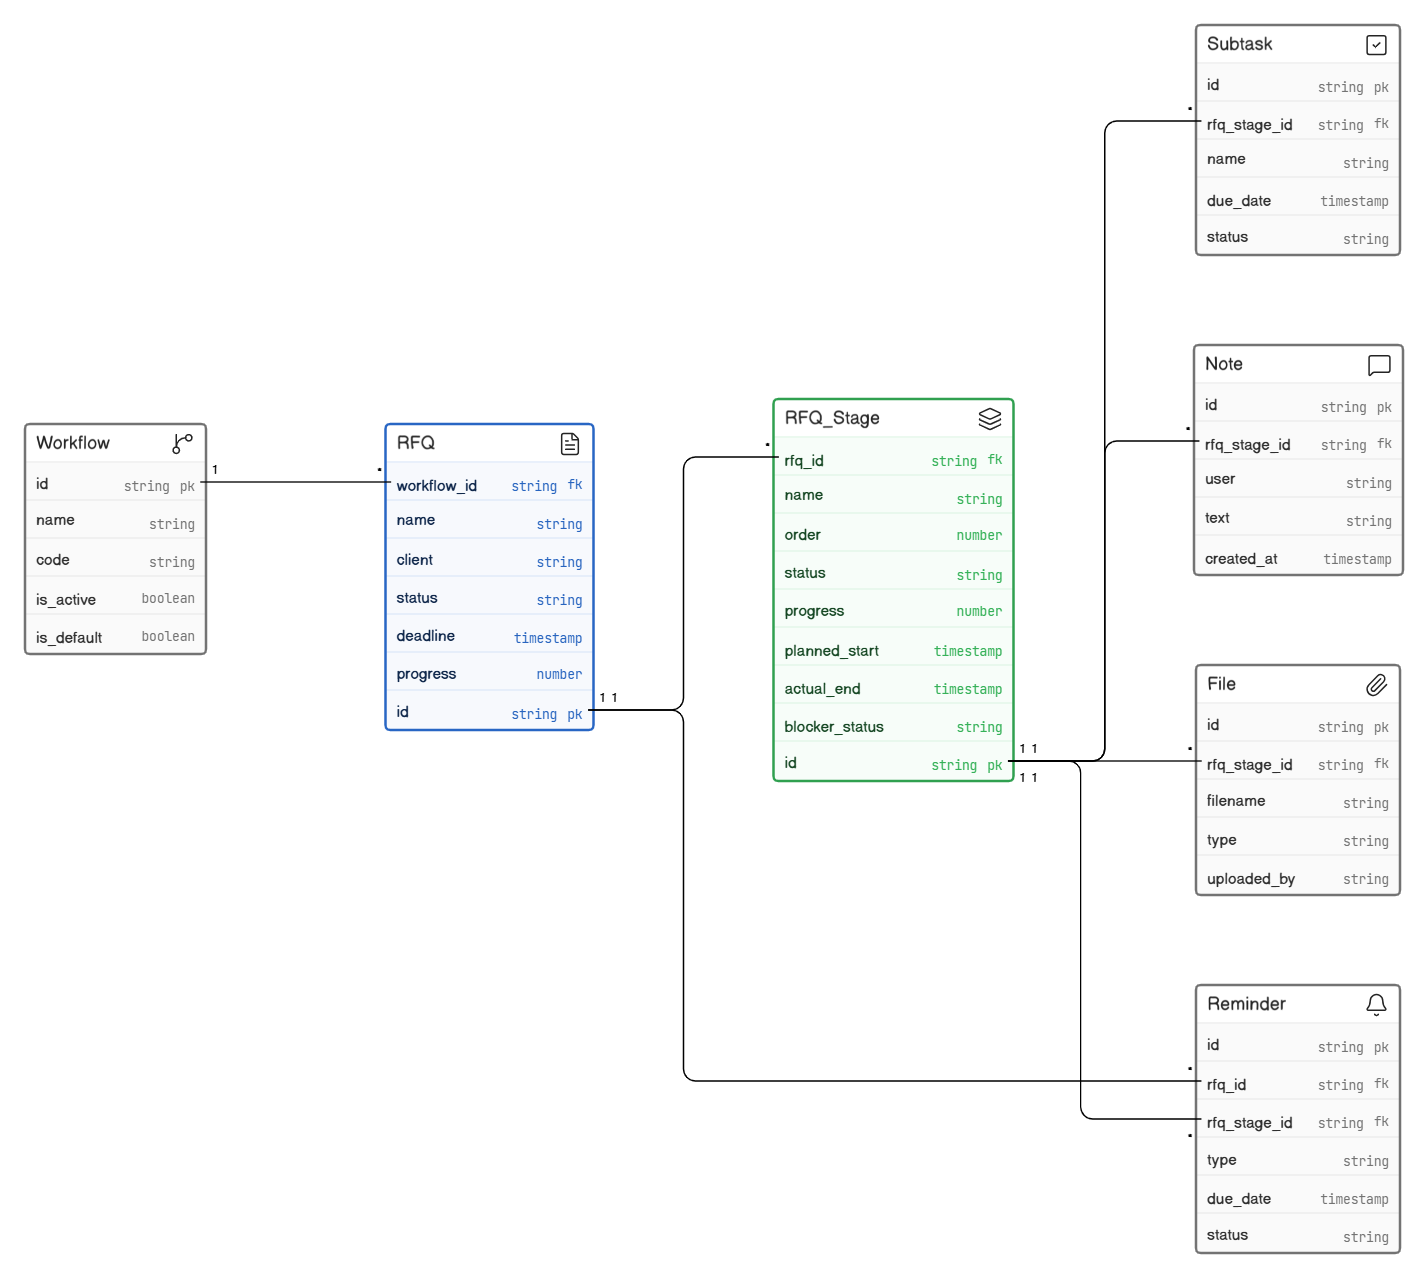
\includegraphics[width=\linewidth]{images/fig_4_3_manager_erd.png}%
        }{%
            \begin{minipage}[c][6cm][c]{14cm}
                \centering
                \textit{[Figure 4.3 placeholder: entity-relationship diagram of the manager service domain model, showing the seven primary entities (RFQ, Workflow, RFQ\_Stage, Subtask, Note, File, Reminder) and their cardinalities.]}
            \end{minipage}%
        }
    }
    \caption{Entity-relationship diagram of the manager service domain model}
    \label{fig:manager_erd}
\end{figure}

\subsection{Workflow and Stage Progression}
The mechanism that gives the manager service its discipline is the stage progression logic. The advance of an RFQ from one stage to the next is a guarded transition: three deterministic gates must be passed (Figure~\ref{fig:three_gates}). The \textit{mandatory-field gate} refuses the advance if any required field of the current stage is missing, returning a structured error identifying the missing fields. The \textit{blocker gate} refuses the advance while structured blocker state on the current stage (raised, for example, by Engineering on a feasibility check) remains unresolved. The \textit{transition-validity gate} refuses any target stage other than the one computed from the workflow template, preventing skipped or out-of-order stages. When all three gates pass, the stage-advance transaction commits atomically from the caller's perspective: the current stage is marked complete with a timestamp, the next stage is activated, the RFQ's overall progress is recomputed, and lifecycle timestamps and persisted stage state are updated in a traceable way. A related concurrency limitation on RFQ-code generation under load (recorded as LG-06 and consolidated in Chapter~6 (Section~6.8)) sits outside the stage-advance transaction and does not affect this atomicity guarantee. The implementation of the three gates in the controller layer is presented in Chapter~5.

\begin{figure}[H]
    \centering
    \setlength{\fboxsep}{5pt}
    \setlength{\fboxrule}{0.5pt}
    \fbox{
        \IfFileExists{images/fig_4_4_three_gates.png}{%
            \includegraphics[width=0.85\linewidth]{images/fig_4_4_three_gates.png}%
        }{%
            \begin{minipage}[c][6cm][c]{12cm}
                \centering
                \textit{[Figure 4.4 placeholder: three-gate activity flow for \textit{Advance RFQ Stage}. Sequential decision diamonds (mandatory-field gate $\rightarrow$ blocker gate $\rightarrow$ transition-validity gate) with halt-on-failure branches returning structured errors, and a single commit branch for the all-pass case that atomically marks the stage complete, activates the next stage, and recomputes RFQ progress.]}
            \end{minipage}%
        }
    }
    \caption{Activity flow of the three-gate stage-progression logic in the manager service}
    \label{fig:three_gates}
\end{figure}

\subsection{Reminder Ownership and API Contract}
Reminders remain inside the manager service because they are tightly coupled to lifecycle artifacts (decision recorded in Appendix~A.10). The manager exposes a versioned REST API organised around seven resource families (RFQ, Workflow, RFQ\_Stage, Subtask, File, Note, Reminder), with around thirty-one endpoints. Three carry particular architectural significance: \textit{advance stage} exercises the three-gate progression logic above; \textit{add note} is append-only by contract, preserving the communication trail; and \textit{upload file} distinguishes file types, including a designated workbook type prepared for downstream intelligence parsing through manual/direct trigger paths. The full API surface is developed in Chapter~5.

\section{Copilot Service: Trust-Boundary Architecture}

The copilot is not an autonomous agent. The language model understands and writes language, but deterministic code decides what data can be used, which tool can run, whether the user may access the RFQ, and what answer is safe to return.

The RFQ Copilot is the conversational layer through which authorised users interact with the platform in natural language, with enforced evidence boundaries and test-backed trust-boundary controls around what it is permitted to do. This section presents the design philosophy, positions the copilot against alternative conversational AI patterns, and develops the trust-boundary architecture that organises its internal logic. The implementation in code is the subject of Chapter~5.

\subsection{Design Philosophy}
The copilot was designed under a single guiding principle, which determines every subsequent architectural choice in this section.

\begin{center}
\fbox{\parbox{0.92\textwidth}{\centering\textit{The copilot should feel like ChatGPT in fluidity, but must not behave like generic ChatGPT in authority. Its authority comes from platform evidence, not from the language model.}}}
\end{center}

This principle separates two qualities typically conflated in conversational systems. \textit{Fluidity} is what makes a system pleasant to interact with: natural language understanding, contextually appropriate replies, the ability to follow a thread across turns. \textit{Authority} is what makes a system safe to act on: claims grounded in real data, scope bounded, behaviour predictable. A generic conversational system optimises for fluidity and produces authority as a fluent-sounding side effect --- precisely what the audit findings of Chapter~1 warned against in an industrial estimation context. The copilot is therefore designed so that fluidity is provided by the language model while authority is owned by deterministic platform components.

\subsection{Positioning Against Alternative Conversational AI Patterns}
The three families surveyed in Chapter~2 (§2.3) --- naive RAG, generic LLM agents, and uncontrolled tool-calling chatbots --- share a structural limitation under cost-of-error-asymmetric conditions: each grants the language model authority over a decision (drift beyond retrieved evidence, tool selection, intent classification) that should remain deterministic. The trust-boundary architecture below adopts a different allocation: language tasks (interpretation, composition, verification) stay with the model; policy tasks (selection, authorisation, escalation) move to deterministic platform components.

\subsection{The Eight Trust Boundaries}
The trust-boundary architecture separates classification from execution through a single deterministic chokepoint and verifies the resulting answer through deterministic guardrails followed by a final language-model judge. It rests on eight decisions, each consciously assigned to a specific owner. Table~\ref{tab:trust_boundaries} presents the eight boundaries.

\begin{table}[H]
\centering
\renewcommand{\arraystretch}{1.4}
\begin{tabular}{|p{0.6cm}|p{6cm}|p{7cm}|}
\hline
\rowcolor{lightgray}
\textbf{\#} & \textbf{Decision} & \textbf{Owner} \\ \hline
1 & What path does this turn belong to? & FastIntake (deterministic) or LLM Planner (proposes), validated by PlannerValidator and decided by ExecutionPlanFactory. \\ \hline
2 & Who may construct an executable plan for a turn? & ExecutionPlanFactory only; single-construction discipline protected by anti-drift tests in the copilot pytest suite. \\ \hline
3 & Which tools are permitted, and which actually run? & Path Registry (mapping) and the deterministic Tool Executor (invocation). \\ \hline
4 & May this user read this RFQ? & The manager service API: a \texttt{404} or \texttt{403} response is the answer, never overridden by the copilot. \\ \hline
5 & Which fields are allowed to enter the language model prompt? & Per-path field whitelist defined in the Path Registry, enforced by the ExecutionPlanFactory. \\ \hline
6 & Which target does each field of evidence belong to? & Per-target labelling at the moment of evidence-packet construction. \\ \hline
7 & Did the response hallucinate, drift in scope, or leak across targets? & Deterministic Guardrails (multiple, sequential), followed by an LLM Judge as the final line of defense. \\ \hline
8 & What happens when any stage fails? & The Escalation Gate, a single deterministic intercept point that re-enters the ExecutionPlanFactory with a structured \texttt{reason\_code}. \\ \hline
\end{tabular}
\caption{The eight trust boundaries of the copilot architecture and their owners}
\label{tab:trust_boundaries}
\end{table}

The eight boundaries can be summarised in one sentence used throughout the project as a quick test of architectural correctness: \textit{two classification sources, one plan factory, one escalation gate; the language model produces language, code produces truth, policy enforces boundaries, the Judge verifies, templates render the safe answer when nothing else worked.} If a proposed change to the system would violate any clause of this sentence, it is the change that is wrong, not the architecture. Figure~\ref{fig:canonical_pipeline} presents the canonical pipeline that realises this architecture, with components coloured by trust class.

\begin{figure}[H]
    \centering
    \setlength{\fboxsep}{5pt}
    \setlength{\fboxrule}{0.5pt}
    \fbox{
        \IfFileExists{images/fig_4_5_canonical_pipeline.png}{%
            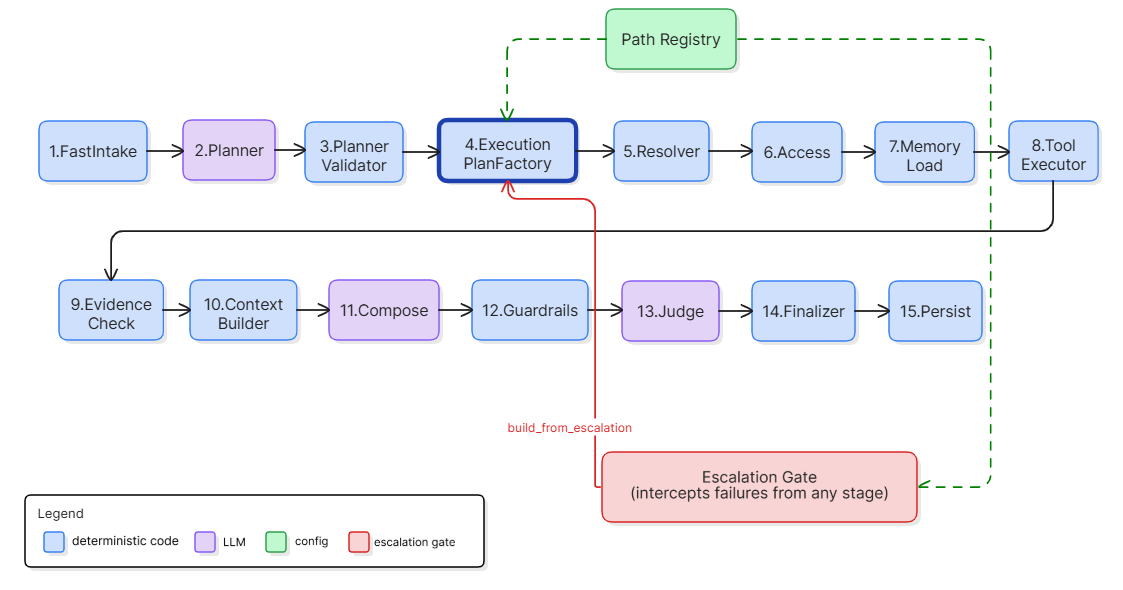
\includegraphics[width=\linewidth]{images/fig_4_5_canonical_pipeline.png}%
        }{%
            \begin{minipage}[c][9cm][c]{14cm}
                \centering
                \textit{[Figure 4.5 placeholder: canonical pipeline of the RFQ Copilot. Thirteen stages (FastIntake $\rightarrow$ Planner $\rightarrow$ PlannerValidator $\rightarrow$ ExecutionPlanFactory $\rightarrow$ Resolver $\rightarrow$ Access $\rightarrow$ Memory Load $\rightarrow$ Tool Executor $\rightarrow$ Evidence Check $\rightarrow$ Context Builder $\rightarrow$ Compose $\rightarrow$ Guardrails $\rightarrow$ Judge $\rightarrow$ Finalizer $\rightarrow$ Persist) coloured by trust class: deterministic code (blue), language model (purple, three stages), Path Registry config (indigo, dashed to Factory + Gate only), Escalation Gate intercept (red), external services (green), persistence (amber). The three LLM stages are visibly bracketed by deterministic stages on either side.]}
            \end{minipage}%
        }
    }
    \caption{Canonical pipeline of the RFQ Copilot, with stages coloured by trust class. The language model (purple) is invoked only at Planner, Compose, and Judge, each bracketed by deterministic stages.}
    \label{fig:canonical_pipeline}
\end{figure}

\subsection{Two Classification Sources, One Plan Factory}
Every user turn enters the copilot through one of two classification sources, both feeding a single point of plan construction; the architecture forbids any third entry path. \textbf{FastIntake} is a deterministic component that recognises trivial messages (greetings, thanks, farewells, pure nonsense) through anchored regular expressions and produces an \texttt{IntakeDecision} without invoking the language model. The \textbf{LLM Planner} is a structured-output language-model invocation that classifies the turn into a supported path and proposes the relevant intent topic, target candidates, and field references; it emits a \texttt{PlannerProposal}, which the \textbf{PlannerValidator} converts to a \texttt{ValidatedPlannerProposal} through structural validation only --- the validator catches malformed output and schema violations but does not enforce policy or read the Path Registry. Both sources feed the \textbf{ExecutionPlanFactory}, the single component in the entire system permitted to construct a \texttt{TurnExecutionPlan}. This discipline is enforced by an anti-drift test that inspects the syntax tree of \texttt{src/pipeline/} and \texttt{src/controllers/} to assert no construction site for \texttt{TurnExecutionPlan} exists outside the factory --- a static structural guard, not a runtime check. The factory reads the Path Registry, applies source-aware policy enforcement, and either produces a valid plan or returns a structured rejection that routes through the Escalation Gate, which calls the same factory through a separate entry point to construct a Path~8 safe plan.

\subsection{The Path Registry as Policy-as-Configuration}
The Path Registry holds the entire policy surface of the copilot in a structured, declarative form. It is read at runtime only by the ExecutionPlanFactory and the Escalation Gate; no other component reads it, an invariant similarly protected by anti-drift tests. For each (path, intent topic) combination it defines: permitted intake sources, authorised evidence tools, allowed/forbidden fields, target resolver strategy, access policy, active guardrails, Judge policy and triggers, memory policy, persistence policy, finalizer template keys, and model profile. Every operational decision the copilot makes flows from this configuration; adding a new path is a configuration change, not a modification of pipeline stages or factory logic.

\subsection{The Pipeline and the Five Evidence Sources}
A user turn that produces an answer flows through a deterministic pipeline of intake $\rightarrow$ factory $\rightarrow$ resolver $\rightarrow$ access $\rightarrow$ memory load $\rightarrow$ tool executor $\rightarrow$ evidence check $\rightarrow$ context builder $\rightarrow$ compose $\rightarrow$ guardrails $\rightarrow$ judge $\rightarrow$ finalizer $\rightarrow$ persist, with the language model invoked only at the Planner, Compose, and Judge stages, each bracketed by deterministic stages on either side (Figure~\ref{fig:canonical_pipeline}). Each stage owns a single decision; the implementation is presented in Chapter~5. Five evidence sources are recognised: the \textbf{conversation itself} for trivial messages; \textbf{manager service state} (dominant in current scope, accessed through the manager connector); \textbf{intelligence service artifacts} (architecturally supported, connector deferred to the Path~5 slice); \textbf{controlled domain knowledge} (a future source for standards questions through a bounded RAG surface); and the \textbf{absence of an answer} (handled by the Path~8 family --- refuse rather than approximate).

\subsection{Memory Architecture}
The copilot captures bounded working memory within the active conversation thread: the most recent turns of the current conversation, bounded by the active path's policy, persisted as part of the per-turn execution record. Two extensions are recognised as future work and excluded from current validated scope: first, the injection of working memory into the Planner, Compose, and Judge prompts; second, an episodic-memory extension across sessions, in which prior conversations on the same target would be condensed for future turns. The present non-injection posture is enforced by a dedicated anti-drift test.

\subsection{Path Coverage in the Present Work}
The architecture supports seven answer paths plus a Path~8 family of five protected sub-cases; Table~\ref{tab:path_coverage} summarises which paths are active in the present work. The coverage strategy exercises every component of the pipeline end-to-end on real operational paths, while Path~8 ensures that every turn --- including those whose answer paths are not yet ready --- terminates in a bounded, deterministic, defensible response.

\begin{table}[H]
\centering
\renewcommand{\arraystretch}{1.3}
\scriptsize
\begin{tabularx}{\textwidth}{|p{2.4cm}|>{\RaggedRight\arraybackslash}X|p{3.5cm}|}
\hline
\rowcolor{lightgray}
\textbf{Path} & \textbf{Description} & \textbf{Status in present work} \\ \hline
Path~1 & Trivial conversational messages (greetings, thanks, farewells) via FastIntake & Active (foundation slice) \\ \hline
Path~4 & RFQ-grounded operational retrieval --- one RFQ, manager-mediated evidence & Active (demo-defining slice) \\ \hline
Path~8 family & Five protected sub-cases: 8.1 unsupported, 8.2 out-of-scope, 8.3 clarification, 8.4 inaccessible, 8.5 no-evidence / source-down / LLM-down & Active (safety net) \\ \hline
Paths~2, 3, 5, 6, 7 & Domain knowledge, portfolio retrieval, intelligence retrieval, cross-RFQ reference, comparison & Short-circuit through the Escalation Gate to Path~8.1 until their slices ship \\ \hline
\end{tabularx}
\caption{Path coverage in the present work}
\label{tab:path_coverage}
\end{table}

\subsection{Why This Architecture Is the Innovation of the Project}
The trust-boundary architecture is the central engineering contribution of this work and the property that distinguishes the platform from a prototype: it is enforced by tests, not by review discipline alone. Three reasons support this claim. \textit{Structural:} the language model is separated from the deterministic platform at the type level (the three-type contract \texttt{IntakeDecision} / \texttt{ValidatedPlannerProposal} / \texttt{TurnExecutionPlan}) and at the test level (anti-drift tests on factory-only construction and registry-reader allowlist) --- self-defending in a way that policy-by-convention is not. \textit{Operational:} every consequential decision is allocated to a component whose behaviour is observable, auditable, and changeable independently of the language model: the Path Registry as configuration, the Tool Executor as code, the Guardrails as testable functions, the Judge through structured logs. \textit{Academic:} the architecture offers an implementable answer to a question the field has not settled --- how should an LLM-driven system behave when the cost of being wrong is high? --- and allocates risk to components designed to handle it.

\section{Evidence Boundary}

The \textit{evidence boundary} is the architectural commitment that the set of evidence sources from which the copilot may reason is finite, named, and decided before the language model is invoked. It operates at two levels. At the \textit{path level}, the boundary determines which sources are legal for a given turn: an operational question about an RFQ may draw from manager state (and from intelligence artifacts when wired for the active path), not from controlled domain knowledge; a standards question may draw from controlled domain knowledge, not from operational state; a greeting requires no evidence at all. The Path Registry encodes this correspondence statically and the ExecutionPlanFactory enforces it at plan-construction time. At the \textit{turn level}, the per-path field whitelist and the per-target labelling discipline introduced in Section~4.4 govern which fields, from which targets, enter the language model's context.

\subsection{Why the Boundary Is Enforceable}
Three architectural properties make the evidence boundary enforceable rather than declarative. First, the \textit{policy-as-configuration} discipline of the Path Registry: every authorised source for every (path, intent topic) is named in configuration that the ExecutionPlanFactory reads before plan construction; a turn for which no source is authorised cannot be assembled and is routed to Path~8. Second, the \textit{single-construction} discipline: the factory is the only component permitted to assemble an executable plan, and it reads the Path Registry --- an invariant protected by anti-drift tests. Third, the \textit{deterministic guardrail and LLM Judge layer}: after the model has composed a draft, guardrails check evidence grounding, scope adherence, and shape conformance; the Judge then performs a final verification on language-level risks (fabrication, scope drift, forbidden inference) that deterministic rules cannot reliably catch. The Judge is the last line of defence, not the first.

\section{Platform Integration and ADR Summary}

\subsection{Platform Integration}
The user interface consumes the manager's lifecycle and analytical endpoints, exposes the copilot at portfolio and per-RFQ levels, and surfaces the intelligence service's parsed profiles, briefings, and anomaly flags in the RFQ detail experience. The intelligence service participates at artifact arrival (manual/direct trigger; autonomous event-driven cascade deferred) and at retrieval (UI fetches persisted profiles through the read API). The copilot's consumption of intelligence artifacts is architecturally supported but not wired in the present implementation. No service is the secondary owner of another service's domain data.

\subsection{Architectural Decisions}
The architectural decisions presented in the preceding sections were not the only options considered. The major decisions made during the project --- service decomposition (monolith vs.\ microservices), intra-service pattern (free-form vs.\ MVC vs.\ BACAB layered), operational source of truth (distributed vs.\ owned by the manager service), reminder ownership (inside the manager service vs.\ a separate communication scope), conversational design (generic LLM agent vs.\ naive RAG vs.\ trust-bound copilot), policy surface (in-code policy vs.\ policy-as-configuration via the Path Registry), plan construction (multiple constructors vs.\ single ExecutionPlanFactory), and identity-and-access management (in-service shim vs.\ dedicated IAM service deferred) --- are recorded in Appendix~A.10 (Table~\ref{tab:decisions}), each with the alternatives considered, the option chosen, the rationale, and the principal consequence accepted.

The most consequential of these is the trust-boundary architecture of the copilot (Section~4.4): it determines the entire shape of the conversational layer and the discipline that governs it.

\section*{CONCLUSION}
\addcontentsline{toc}{section}{CONCLUSION}
This chapter has presented the conceptual and technical architecture of Itqan: the four-layer platform with the copilot positioned as a cross-cutting interaction layer, the four-pillar capability map, the five-service inventory with one service kept as future scope, the BACAB pattern realised across the backend services, the manager service backbone with its three-gate lifecycle, the trust-boundary architecture of the copilot, the evidence boundary that governs copilot reasoning over platform data, and the platform-integration view and architectural-decision register. Chapter~5 develops the implementation of this architecture in code; Chapter~6 presents the validation evidence used to verify how these trust boundaries are preserved in the implemented system.